% Chapter 3

\chapter{ Finite element algorithms for contact problems \parencite{CONTACTBOOK} \parencite{ref4} } % Main chapter title

\label{Chapter4} % For referencing the chapter elsewhere, use \ref{Chapter1} 

%----------------------------------------------------------------------------------------

\section{Introduction}
Boundary value problems involving contact are of great importance in industrial applications
in mechanical and civil engineering. The range of application includes metal forming
processes, drilling problems, bearings, crash analysis of cars, car tires or cooling of electronic
devices. Other applications are related to biomechanics where human joints, implantats or
teeth are of consideration. Due to this variety contact problems are today combined either
with large elastic or inelastic deformations including time dependent responses. Thermal
coupling might have to be considered, see the cooling of electronic devices, the heat removal
within nuclear power plant vessels or thermal insulation of astronautic vehicles. Even
stability behaviour has to be linked to contact, like wrinkling arising in metal forming
problems.

Due to this technical importance a great number of researchers have investigated contact
problems. In the ancient egypt people needed to move large stone blocks to build the
pyramids and thus had to overcome the frictional force associated with it. Thus many known
researchers in the past have investigated frictional contact problems, amongst them were
Da Vinci, Amontons, Newton, Coulomb. Their investigations were based on the assumption
of rigid bodies. Starting with the classical analytical work of Hertz (1882) on the elastic
contact of two spheres the deformation of the bodies being in contact has been taken into
account. However only very few problems involving contact can be solved analytically. Thus
for most industrial applications numerical methods have to be applied when the contacting
bodies have complex geometries . Due to that the solution of contact problems with finite
element methods has a relatively long history, see Wilson, Parsons (1970) or Chan, Tuba
(1971) for early treatments.

In this overview article we will restrict ourselves mainly to finite element techniques for
the treatment of contact problems despite many other numerical schemes and analytical
approaches could be discussed as well. Furthermore we like to note that the description
of the mechanical behaviour of the bodies coming into contact will not be investigated in
detail, although this is of great importance. This article thus concentrates on the behaviour
in the contact interface. The associated formulation and discretization within the finite
element method will be considered as well as the development of algorithms.
\section{Contact Geometry}
This section summarizes relations which are necessary to formulate the geometrical contact
conditions. In detail the penetration and the relative slip in the contact area are discussed.
The first condition also includes the non–penetration condition which is used classically in
contact mechanics.

We assume that two bodies which undergo large deformations can come into contact.
Let $\mathcal{B}^\gamma$ , $ \gamma= 1, 2$ , denote the two bodies of interest and $\boldsymbol{\varphi}_{t}^{\gamma}: \mathcal{B}^{\gamma} \rightarrow \mathbb{R}^{3}$ the associated
deformation maps at time $t \in \mathbb{R}$. $\phi_t^{\gamma}$ maps points $\boldsymbol{X}^\gamma \in \mathcal{B}^\gamma$ of the reference configuration
onto points $x^\gamma = \phi ^\gamma_t(X^\gamma)$ of the current configuration.

%---------------------------------------------------
\section{Penetration}
As the first relevant function for the contact geometry we define a penetration function on
the current slave surface $\phi _t^1(\Gamma_c^1)$ by setting
\begin{equation}
 g_{N+}=\left\{\begin{array}{ll}\left\|\mathbf{x}^{1}-\hat{\mathbf{x}}_{t}^{2}\left(\bar{\xi}^{1}, \bar{\xi}^{2}\right)\right\| & \text { for }\left[\mathbf{x}^{1}-\hat{\mathbf{x}}_{t}^{2}\left(\bar{\xi}^{1}, \bar{\xi}^{2}\right)\right] \cdot \overline{\mathbf{n}}^{2}<0 \\ 0 & \text { otherwise }\end{array}\right. 
 \label{eqn:4.1} 
\end{equation}

Here $(\hat{\xi}^1,\hat{\xi}^2)$ is the minimizer of the distance function for a given slave point $x^1$
\begin{equation}
 \hat{d}^{1}\left(\xi^{1}, \xi^{2}\right)=\left\|\mathbf{x}^{1}-\hat{\mathbf{x}}_{t}^{2}\left(\xi^{1}, \xi^{2}\right)\right\| \longrightarrow \mathrm{MIN} 
 \label{eqn:4.2} 
\end{equation}

The values  $(\hat{\xi}^1,\hat{\xi}^2)$ are obtained by writing the necessary condition for the minimum of
the distance function (\ref{eqn:4.2})
\begin{equation}
 \frac{d}{d \xi^{\alpha}} \hat{d}^{1}\left(\xi^{1}, \xi^{2}\right)=\frac{\mathbf{x}^{1}-\hat{\mathbf{x}}_{t}^{2}\left(\xi^{1}, \xi^{2}\right)}{\left\|\mathbf{x}^{1}-\hat{\mathbf{x}}_{t}^{2}\left(\xi^{1}, \xi^{2}\right)\right\|} \cdot \hat{\mathbf{x}}_{t, \alpha}^{2}\left(\xi^{1}, \xi^{2}\right)=0
 \label{eqn:4.3} 
\end{equation}

The solution of (\ref{eqn:4.3}) requires the orthogonality of the first and second term. Since
$ \hat{\mathbf{x}}_{t, \alpha}^{2}\left(\xi^{1}, \xi^{2}\right) 
$  is the tangent vector $a^_\alpha$ the first term must denote the normal $n^2$ . Thus we
have the condition $-n^2 \cdot a^2_\alpha=0$ which means that the current master point $ \hat{\mathbf{x}}_{t}^{2}\left(\xi^{1}, \xi^{2}\right) 
$ is
the orthogonal projection of a given slave point $x^1$ onto the current master surface $\phi_t^2(\Gamma^2_c)$ .

Here and in the following we will denote by a bar over a quantity its evaluation at the
minimal distance point $\left(\overline{\xi}^{1}, \overline{\xi}^{2}\right)$ which means that these values denote the solution point of
(\ref{eqn:4.3}). Thus $\overline{\mathbf{n}}^{2}:=\left(\overline{\mathbf{a}}_{1}^{2} \times \overline{\mathbf{a}}_{2}^{2}\right) /\left\|\overline{\mathbf{a}}_{1}^{2} \times \overline{\mathbf{a}}_{2}^{2}\right\|$ is the outward unit normal on the current master
surface at the master point where $\overline{a}_\alpha^2$ are tangent vectors at $\hat{\mathbf{x}}_{t}^{2}\left(\overline{\xi^{1}}, \overline{\xi^{2}}\right)$.

The penetration function (\ref{eqn:4.1}) contains two informations:
\begin{enumerate}
    \item $g_{N+} $ serves as a local contact check, i.e. we set: $\text{contact} \Leftrightarrow	 g_{ N + }> 0$
    \item  $g_{N+} $ enters for $g_{N+} > 0$as a local kinematical variable the constitutive function for the contact pressure.
\end{enumerate}

By taking the time derivative of (\ref{eqn:4.2}) at the minimal distance point $\left(\overline{\xi}^{1}, \overline{\xi}^{2}\right)$ ) one obtains,
in the case of contact, the rate of penetration
\begin{equation}
 \dot{g}_{N+}=\left[\mathbf{v}_{t}^{1}-\hat{\mathbf{v}}_{t}^{2}\left(\bar{\xi}^{1}, \bar{\xi}^{2}\right)\right] \cdot \overline{\mathbf{n}}^{2} 
 \label{eqn:4.4} 
\end{equation}
for given spatial velocities $v_t^1 $ and $\hat{v}_t^2\left(\overline{\xi}^{1},\overline{\xi}^{2}\right)$  at the slave and master points.
%------------------------------------------------------------------------------
\section{Tangential Relative Velocity and Tangential Relative Slip}
The tangential relative slip between two bodies is related to the change of the solution point
$( \overline{\xi}^1 , \overline{\xi}^2)$ of the minimal distance problem. Thus we can compute the time derivative of $\xi^ \alpha$
from (\ref{eqn:4.3}). This yields the following result 
\begin{equation}
 \frac{d}{d t}\left\{\left[\mathbf{x}_{t}^{1}-\hat{\mathbf{x}}_{t}^{2}\left(\bar{\xi}^{1}, \bar{\xi}^{2}\right)\right] \cdot \overline{\mathbf{a}}_{\alpha}^{2}\right\}=\left[\mathbf{v}_{t}^{1}-\hat{\mathbf{v}}_{t}^{2}\left(\bar{\xi}^{1}, \bar{\xi}^{2}\right)-\overline{\mathbf{a}}_{\beta}^{2} \dot{\overline{\xi}}^{\beta} \right] \cdot \overline{\mathbf{a}}_{\alpha}^{2}+\left[\mathbf{x}_{t}^{1}-\hat{\mathbf{x}}_{t}^{2}\left(\bar{\xi}^{1}, \bar{\xi}^{2}\right)\right] \cdot \dot{\overline{\mathbf{a}}}_{\alpha}^{2}=0 
 \label{eqn:4.7} 
\end{equation}
with $\dot{\overline{{\mathbf{a}}}}_{\alpha}^{2}=\hat{\mathbf{v}}_{t, \alpha}^{2}\left(\bar{\xi}^{1}, \bar{\xi}^{2}\right)+\hat{\mathbf{x}}_{t, \alpha \beta}^{2}\left(\bar{\xi}^{1}, \overline{\xi}^{2}\right) \dot{\overline{\xi}}^{\beta} $ we obtain $\dot{\overline{\xi}}^{\beta} $ from the following system of equations
\begin{equation}
    \label{eqn:4.8} 
    \overline{H}_{\alpha \beta } \dot{\overline{\xi}}^{\beta} =\overline{R}_\alpha
\end{equation}
with 
\begin{equation}
 \begin{aligned} \overline{H}_{\alpha \beta} &=\left[\bar{a}_{\alpha \beta}+g_{N+} \overline{b}_{\alpha \beta}\right] \\ \overline{R}_{\alpha} &=\left[\mathbf{v}_{t}^{1}-\hat{\mathbf{v}}_{t}^{2}\left(\overline{\xi}^{1}, \overline{\xi}^{2}\right)\right] \cdot \overline{\mathbf{a}}_{\alpha}^{2}+g_{N+} \overline{\mathbf{n}}^{2} \cdot \hat{\mathbf{v}}_{t, \alpha}^{2}\left(\overline{\xi}^{1}, \overline{\xi}^{2}\right) \end{aligned} 
 \label{eqn:4.9} 
\end{equation}

$\bar{a}_{\alpha \beta}$ and $\overline{b}_{\alpha \beta}$  are the first and second fundamental form of the deformed surface, well known
from differential geometry.

Let us now define the tangential relative velocity function on the current slave surface $\varphi^1_t(\Gamma_c^1)$ by setting
\begin{equation}
 \mathcal{L}_{v} \mathbf{g}_{T}:={\dot{\overline{\xi}^{\alpha}}} \overline{\mathbf{a}}_{\alpha}^{2} 
 \label{eqn:4.10} 
\end{equation}

Equation (\ref{eqn:4.10}) determines per definition the evolution of the tangential slip $g_T$ which
enters as a local kinematical variable the constitutive function for the contact tangential
stress, see next section. The rate \dot{\overline{\xi}^{\alpha}} in (\ref{eqn:4.1}) at the solution point $( \overline{\xi}^ 1 , \overline{\xi}^ 2 )$ has been already
computed in (\ref{eqn:4.8}).
%------------------------------------------------------------------------------
\section{Boundary Value Problem, Global Solution Strategies}
For the formulation of the boundary value problem we have to discuss only the additional
terms due to contact in detail. The equations describing the behaviour of the bodies coming
into contact do not change. However, for completeness, the balance equations and a simple
constitutive model are stated for elastic solids undergoing finite deformation.
\subsection{Local Balance Equations for the Solid}
We can formulate the local momentum equation for a body $\mathcal{B}^\gamma$ as

\begin{equation}
 \operatorname{DIV} \mathbf{P}^{\gamma}+\overline{\mathbf{f}}^{\gamma}=\mathbf{0} 
 \label{eqn:4.24} 
\end{equation}
in case that inertia terms are neglected. $P^\gamma$ denotes the first Piola–Kirchhoff stress tensor acting in the body $\gamma,\overline{f}^\gamma$ are the body forces. Next we formulate the boundary conditions
for the deformation and the stress field
\begin{equation}
 \begin{aligned} \boldsymbol{\varphi}^{\gamma} &=\overline{\boldsymbol{\varphi}}^{\gamma} & & \text { on } \quad \Gamma_{\varphi}^{\gamma} \\ \mathbf{t}^{\gamma} &=\overline{\mathbf{t}}^{\gamma} & & \text { on } \quad \Gamma_{\sigma}^{\gamma} \end{aligned} 
 \label{eqn:4.25} 
\end{equation}

where $\overline{\boldsymbol{\varphi}}$ and $\overline{\mathbf{t}}^{\gamma} $  are described quantities. Furthermore we have to account for the contact
condition which is given  with the definition of the gap function (\ref{eqn:4.1}) when
an approach of the bodies in the contact interface is allowed or by the condition which yields the inequality
\begin{equation}
     g_{N+}^{L} \geq 0 \quad  on  \quad \Gamma_{c} 
     \label{eqn:4.26} 
\end{equation}
%--------------------------------------------------------------------------
\subsection{Constitutive Relations}

As a model for non–linear constitutive equations we use a form valid for finite elasticity which
leads to a non–linear relation between the Kirchhoff stress $\tau$ and the left Cauchy Green tensor
$ b = F F^ T : \tau = f ( b )$. The Kirchhoff stress is related to the first Piola–Kirchhoff stress via
$\tau = P F ^T$ , with $F$ being the deformation gradient. The simplest constitutive equation for
hyperelasticity is known as the Neo–Hookian model and can e. g. be applied for rubber
materials undergoing moderately large strains, see e.g. Ogden (1984). It is stated below for
the body $\mathcal{B}^\gamma$ with the Jacobian of the deformation $J ^ \gamma = det F ^\gamma$

\begin{equation}
    \label{eqn:4.27} 
     \boldsymbol{\tau}^{\gamma}=\Lambda^{\gamma}\left(J^{\gamma}-1\right) \mathbf{1}+\mu^{\gamma}\left(\mathbf{b}^{\gamma}-\mathbf{1}\right).
\end{equation}

Material parameters for the body $\mathcal{B}^\gamma$ are the Lame constants $\Lambda^\gamma$ and $\nu^\gamma$ . The material
model is valid for finite elastic deformations. Of course we can consider more complicated
constitutive relations which can also be of inelastic nature. It should be noted that since the
contact has to be formulated only within the interface, the constitutive laws for the bodies coming into contact can be arbitrary and do not affect the main algorithmic treatment of
the contact problem. However it is clear that the physical properties of the surfaces of the
bodies are influenced by the general constitutive behaviour.
%--------------------------------------------------------------------
\subsection{Weak Formulation}

For a numerical solution of the nonlinear boundary value problem summarized above we
will use the finite element method. Thus we need the weak form of equations (\ref{eqn:4.24}) to (\ref{eqn:4.27}).
Due to the fact that the constraint condition (\ref{eqn:4.24}) is represented by an inequality we obtain
in general a variational inequality. The general form can be written as
\begin{equation}
 \sum_{\gamma=1}^{2} \int_{\Omega^{\gamma}} \boldsymbol{\tau}^{\gamma} \cdot \operatorname{grad}\left(\boldsymbol{\eta}^{\gamma}-\boldsymbol{\varphi}^{\gamma}\right) d V \geq \sum_{\gamma=1}^{2} \int_{\Omega^{\gamma}} \overline{\mathbf{f}}^{\gamma} \cdot\left(\boldsymbol{\eta}^{\gamma}-\boldsymbol{\varphi}^{\gamma}\right) d V-\int_{\Gamma_{\sigma} \gamma} \overline{\mathbf{t}}^{\gamma} \cdot\left(\boldsymbol{\eta}^{\gamma}-\boldsymbol{\varphi}^{\gamma}\right) d A 
 \label{eqn:4.28} 
\end{equation}
where the integration is performed with respect to the domain $\Omega^ \gamma$ occupied by the body
$\mathcal{B}^ \gamma $in the reference configuration. The stress tensor and the gradient operator ”grad” are
evaluated with respect to the current coordinates.

We now have to find the deformation $(\varphi^1,\varphi^2)$ such that (\ref{eqn:4.26}a) is fulfilled for all $(\eta^1,\eta^2)$ with
\begin{equation}
 \mathbf{K}=\left\{\left(\boldsymbol{\eta}^{1}, \boldsymbol{\eta}^{2}\right) \in \mathbf{V} \mid\left[\boldsymbol{\eta}^{1}-\hat{\eta}^{2}\left(\bar{\xi}^{1}, \bar{\xi}^{2}\right)\right] \cdot \overline{\mathbf{n}}^{2} \geq 0\right\} 
\end{equation}

The strain energy function has to be polyconvex and the solution lies in the usual Sobolev space $W ^{1,p} $.
The space $V$ is defined as $\mathbf{V}=\left\{\boldsymbol{\eta}^{\gamma} \in\left[W^{1, p}\left(\Omega^{\gamma}\right)\right]^{\operatorname{dim}} \mid \boldsymbol{\eta}^{\gamma}=\mathbf{0} \quad\right. $ on $ \left.\Gamma_{u}\right\}$ , dim denotes the dimension of the problem at hand.

Within an active set strategy we can write the weak form as an equality since we know
the active set within an incremetal solution step. Then equations (\ref{eqn:4.24}) to (\ref{eqn:4.27}) yield
\begin{equation}
     \sum_{\gamma=1}^{2}\left\{\int_{\Omega^{\gamma}} \boldsymbol{\tau}^{\gamma} \cdot \operatorname{grad} \boldsymbol{\eta}^{\gamma} d V-\int_{\Omega ^\gamma} \overline{\mathbf{f}}^{\gamma} \cdot \boldsymbol{\eta}^{\gamma} d V-\int_{\Gamma_{\sigma} \gamma} \overline{\mathbf{t}}^{\gamma} \cdot \boldsymbol{\eta}^{\gamma} d A\right\} 
 + \textit{"Contact Contributions"}  =0
 \label{eqn:4.30} 
\end{equation}

Note that the integration is performed with regard to the reference configuration but the
stress tensor and the gradients are evaluated with respect to current configuration. $\eta^\gamma \in V$
is the so called test function or virtual displacement which is zero at the boundary $\Gamma_\varphi^\gamma$ where
the deformations are prescribed.

For two boform of the interface by assuming that contact is active at the surface $\Gamma_c$ . dies being in contact we obtain the weak Then the formulation follows for the three different
cases as given below.
\begin{enumerate}
    \item \textbf{Lagrangian multiplier method:}
    \begin{equation}
 \int_{\Gamma_{c}}\left(\lambda_{N} \delta g_{N+}^{L}+\lambda_{T} \cdot \delta \mathbf{g}_{T}\right) d A 
 \label{eqn:4.31} 
\end{equation}
Here $\lambda_N$ denotes the Lagrangian multiplier which can be identified as the contact
 pressure $p_N \bulle \epsilon g_{N+}^Lt$ is the variation of the normal gap. The term $\lambda _T \bullet \epsilon g _T $is associated with
the tangential stick or slip motion and needs further discussion. In case of pure stick
the relative tangential slip $g _T$ is zero which yields a constraint equation from which $\lambda _T$
follows as a reaction. In case of sliding the tangential stress vector $t _T$ is determined
by the constitutive law for frictional slip,  thus we should write
instead of $\boldsymbol{\lambda}_{T} \cdot \delta \mathbf{g}_{T} \longrightarrow \mathbf{t}_{T} \cdot \delta \mathbf{g}_{T} $ .

\item \textbf{Penalty method:}
In this formulation a penalty term due to the constraint condition is added to the
weak form (\ref{eqn:4.26}). This means that once the constraint equation for $g_{N+}^L$ is violated
\begin{equation}
 \int_{\Gamma_{c}} \epsilon_{N} g_{N+}^{L} \delta g_{N+}^{L} d A, \quad \epsilon_{N}>0 
    \label{eqn:4.32} 
\end{equation}
has to be considered for normal contact. The solution of the Lagrangian multiplier method can be recovered from this
formulation for $\epsilon_N \rightarrow \infty$, however this will lead to an ill–conditioned problem, see next section. As in the Lagrangian multiplier method we have to distinguish between
pure stick in the contact interface which produces a penalty term also for the tangential
direction
\begin{equation}
 \int_{\Gamma_{c}}\left(\epsilon_{N} g_{N+}^{L} \delta g_{N+}^{L}+\epsilon_{T} \mathbf{g}_{T} \cdot \delta \mathbf{g}_{T}\right) d A, \quad \epsilon_{N}>0, \epsilon_{T}>0 
 \label{eqn:4.33} 
\end{equation}
and the slip condition which leads to
\begin{equation}
 \int_{\Gamma_{c}}\left(\epsilon_{N} g_{N+}^{L} \delta g_{N+}^{L}+\mathbf{t}_{T} \cdot \delta \mathbf{g}_{T}\right) d A, \quad \epsilon>0 
 \label{eqn:4.34} 
\end{equation}

\item \textbf{Constitutive equation in the interface:}
\begin{equation}
 \int_{\Gamma_{c}}\left(p_{N} \delta g_{N}+\mathbf{t}_{T} \cdot \delta \mathbf{g}_{T}\right) d A\label{eqn:4.35} 
\end{equation}
One can easily see, that the introduction of the constitutive equation for the normal pressure
yields a nonlinear penalty functional for the normal contact. The standard penalty method
can be recovered from this relation by using $n = 1$. However this choice is somehow
artificial since the usual range of the constitutive parameter n, stemming from experiments,
is in the range $2   \leq 3.33$.

In equations (\ref{eqn:4.31}) to (\ref{eqn:4.35}) the variation of the normal gap function $g_{N+}$ is needed which
yields
\begin{equation}
 \delta g_{N+}=\left[\boldsymbol{\eta}^{1}-\boldsymbol{\eta}^{2}\left(\bar{\xi}_{1}, \bar{\xi}_{2}\right)\right] \cdot \overline{\mathbf{n}}^{2} 
 \label{eqn:4.36} 
\end{equation}

Furthermore the variation of the tangential slip can be stated as
\begin{equation}
 \delta \mathbf{g}_{T}=\delta \bar{\xi}^{\alpha} \overline{\mathbf{a}}_{\alpha}^{2} 
\label{eqn:4.37} 
\end{equation}
\end{enumerate}

The latter relation follows simply from (\ref{eqn:4.10}) by replacing the velocities $v$ by the test
function $\eta$ in (\ref{eqn:4.9})

\section{Discretization Techniques Within The Contact Area}
The discretization of the domain contributions of the bodies being in contact in (\ref{eqn:4.30}) is not
objective of this work. Within this context we refer to the finite element implementations of
boundary-value-problems regarding finite elasticity. This leads to the following matrix formulation for the weak form (\ref{eqn:4.30})
\begin{equation}
 \mathbf{G}(\mathbf{v})=\sum_{\gamma=1}^{2}\left\{\int_{\mathcal{B}^{\gamma}} \mathbf{B}^{T} \boldsymbol{\tau}^{\gamma} d V-\int_{\mathcal{B}^{\gamma}} \mathbf{N}^{T} \overline{\mathbf{f}}^{\gamma} d V-\int_{\Gamma_{\sigma} \gamma} \mathbf{N}^{T} \overline{\mathbf{t}}^{\gamma} d A\right\} 
 \label{eqn:4.43}
\end{equation}
where the matrix $N$ contains the shape functions and the so–called $B$matrix contains
the derivatives of the shape functions. Any standard finite element book can be used, for
details.

Here we focus on the contact constraints. For reasons of simplicity we will restrict
ourselves here to two dimensional formulations. We like now to discuss different possibilities to discretize the contact
contributions (\ref{eqn:4.31}) to (\ref{eqn:4.35}) and the variations in normal and tangential direction (\ref{eqn:4.36}) and (\ref{eqn:4.37}).

The basic difference between the Lagrangian method (\ref{eqn:4.31}) and the penalty approach (\ref{eqn:4.32})
lies in the fact that the Lagrangian multiplier formulation is a mixed method which means
that both variables $\lambda_N$ and $ \epsilon_{gN}$ have to be discretized.
\begin{equation}
 \int_{\Gamma_{\mathrm{c}}} \lambda_{N} \delta g_{N} d \Gamma \longrightarrow \int_{\Gamma_{c}^{h}} \lambda_{N}^{h} \delta g_{N}^{h} d \Gamma 
 \label{eqn:4.44}
\end{equation}
with the interpolations for $\lambda_{N}^{h}$ and $ \delta g_{N}^{h}$
\begin{equation}
 \lambda_{N}^{h}=\sum_{K} M_{K}(\xi) \lambda_{N K} \quad  \textit{and} \quad \delta g_{N}^{h}=\sum_{I} N_{I}(\xi) \delta g_{N I} 
\end{equation}

In the following we will only discuss discretizations related to the penalty method and
to the formulation using constitutive equations in the contact interface where the contact
pressure follows e.g. via $(\ref{eqn:4.10})$ from the displacement variables.

In general there are different discretizations of $\Gamma_c$ possible which depend on the problem
(linear or nonlinear kinematics), on the discretization of the bodies in contact and on the
type of constitutive interface law. Some discretizations are depicted in Figure \ref{fig:abcd} a) to d).
\begin{figure}[H]
    \centering
    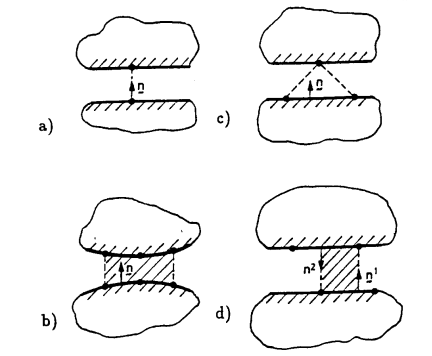
\includegraphics[scale=0.7]{Figure2/Chap4/abcd.png}
    \caption{Different contact discretizations}
    \label{fig:abcd}
\end{figure}
\subsection{Node–to–node Contact Element}
Figure \ref{fig:abcd} a) shows the so-called node–to–node contact which can only be applied to geometrically linear problems since a relative tangential movement of the nodes is not allowed in
the contact area. Due to its simplicity it resolves the integral (\ref{eqn:4.32}) to
\begin{equation}
 \int_{\Gamma_{c}} \epsilon_{N} g_{N} \delta g_{N} d \Gamma \longrightarrow \sum_{i=1}^{n_{c}} \epsilon_{N} g_{N i} \delta g_{N i} A_{i}=\sum_{i=1}^{n_{c}} \epsilon_{N} g_{N i}\left(\boldsymbol{\eta}_{i}^{1}-\boldsymbol{\eta}_{i}^{2}\right) \cdot \mathbf{n}_{i}^{2} A_{i} 
 \label{eqn:4.46}
\end{equation}

where $n _c$ are the contact nodes in $\Gamma^h_c$. The test function $\eta_i^\alpha$ and the normal vector $n^ 2_ i$ is
defined for the node $i$ . Often the area $A_ i$ is neglected
(or ”hidden” in the penalty parameter - $\epsilon_N$ ) in the node–to–node contact formulation which
means that the contact stress $p_N=\epsilon_N g_N$ becomes a contact (nodal) force $f_{Ni}=\epsilon_N g_{Ni}$ .Then an evaluation of a contact interface law is not possible with discretization
(\ref{eqn:4.46}). The associated matrix formulation leads in the geometrically linear case for the contact
element i to the definition of the contact residual $G ^c_i = \xi ^T G^ c_i $ and its associated tangent
matrix $K ^c_i $ with
\begin{equation}
 \mathbf{G}_{i}^{c}=\epsilon_{N} g_{N i} \mathbf{N}_{i}, \quad \mathbf{K}_{i}^{c}=\epsilon_{N} \mathbf{N}_{i} \mathbf{N}_{i}^{T}, \quad  \textit{with}  \quad \mathbf{N}_{i}=\left\{\begin{array}{r}\mathbf{n}_{i}^{2} \\ -\mathbf{n}_{i}^{2}\end{array}\right\} 
\end{equation}

\subsection{Isoparametric Discretization of the Contact Contribution}
In Figure \ref{fig:abcd} b) a contact element is shown which also does not allow a relative tangential
movement in the contact area and thus is only valid for geometrically linear applications.
Within this element the gap function $g_{N+}$ is discretized by an isoparametric interpolations
leading also to a well defined contact pressure. We obtain with the interpolation
\begin{equation}
     g_{N+}^{h}=\sum_{I} N_{I}(\xi) g_{N I} \qquad  \textit{and}  \qquad \delta g_{N+}^{h}=\sum_{I} N_{I}(\xi)\left(\boldsymbol{\eta}_{I}^{1}-\boldsymbol{\eta}_{I}^{2}\right) \cdot \mathbf{n}^{2} 
\end{equation}
the discretization of the contact integral (\ref{eqn:4.32})
\begin{equation}
 \int_{\Gamma_{c}} \epsilon_{N} g_{N} \delta g_{N} d \Gamma \longrightarrow \int_{-1}^{1} \epsilon_{N} g_{N+}^{h}(\xi)\left[\sum_{I} N_{I}(\xi)\left(\boldsymbol{\eta}_{I}^{1}-\boldsymbol{\eta}_{I}^{2}\right) \cdot \mathbf{n}^{2}\right]\left\|\frac{d x^{h}}{d \xi}\right\| d \xi 
 \label{eqn:4.48}
\end{equation}

Finally numerical integration can be applied to evaluate (48). For the proper choice of the
numerical integration rule. This discretization leads to a contact element which
can be applied together with four or nine node quadilaterals for the continuum problem.
Due to the smooth discretization a good approximation of the contact pressure is obtained.
%-----------------------------------------------------------
\subsection{Node–to–segment Contact Discretization}
A more general discretization of the contact interface which allows also for large tangential
sliding is given by the setup depicted in Figure \ref{fig:abcd} c). This discretization is named node–to–segment contact element and is widely used in nonlinear finite element simulations of
contact problems.

Due to its importance we like to consider this contact element in more detail. Assume
that the discrete slave point (s) comes into contact with the master segment (1)–(2), see
Figure 6. With the interpolation for the master segment
\begin{equation}
 \hat{\mathbf{x}}^{2}(\xi)=\mathbf{x}_{1}^{2}+\left(\mathbf{x}_{2}^{2}-\mathbf{x}_{1}^{2}\right) \xi 
 \label{eqn:4.49}
\end{equation}
one can easily compute the tangent vector of the segment leading to
\begin{equation}
 \overline{\mathbf{a}}_{1}^{2}=\hat{\mathbf{x}}^{2}(\xi)_{, 1}=\left(\mathbf{x}_{2}^{2}-\mathbf{x}_{1}^{2}\right) 
 \label{eqn:4.50}
\end{equation}

It is connected to an orthonormal base vector $a ^2_1$  by $a ^2_1 = \overline{a}^2_1 / l $ with $l =\left\| x ^2_2 -  x ^2_1 \right\| $  being
the current length of the master segment. With the unit tangent vector $a ^2_1$ the unit normal
to the segment $(1)–(2)$ can be defined as $n ^2 = e _3 × a ^2_1$ .
\begin{figure}[H]
    \centering
    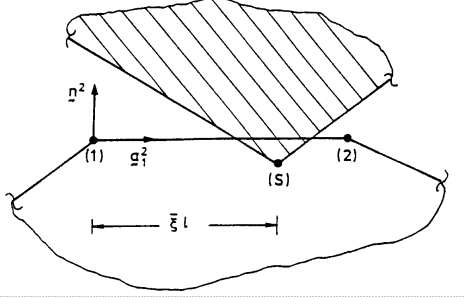
\includegraphics[scale=0.6]{Figure2/Chap4/fig6.png}
    \caption{Node–to–segment element}
    \label{fig4:6}
\end{figure}

$\overline{\xi}$ and $g _N$ are given by the solution of the minimal distance problem by the projection
of the slave node $x_s$ in $(s)$ onto the master segment $(1)–(2$)
\begin{equation}
    \label{eqn:4.51}
     \bar{\xi}=\frac{1}{l}\left(\mathbf{x}_{s}^{1}-\mathbf{x}_{1}^{2}\right) \cdot \mathbf{a}_{1}^{2} \quad  \textit{and}  \quad g_{N s}=\left\|\mathbf{x}_{s}^{1}-(1-\bar{\xi}) \mathbf{x}_{1}^{2}-\bar{\xi} \mathbf{x}_{2}^{2}\right\| 
\end{equation}

From these equations and the local formulation (\ref{eqn:4.4}) we compute directly the variation of the
gap function $\delta^g_{N+}$ on the straight master segment (1)–(2).
\begin{equation}
 \delta g_{N s}=\left[\boldsymbol{\eta}_{s}^{1}-(1-\bar{\xi}) \boldsymbol{\eta}_{1}^{2}-\bar{\xi} \boldsymbol{\eta}_{2}^{2}\right] \cdot \mathbf{n}^{2}
 \label{eqn:4.52}
\end{equation}

The local equation (\ref{eqn:4.9}) yields the expression for $\delta \overline{\xi}$.  With the interpolation for the variation $\hat{\boldsymbol{\eta}}^{2}(\xi)=\boldsymbol{\eta}_{1}^{2}+\xi\left(\boldsymbol{\eta}_{2}^{2}-\boldsymbol{\eta}_{1}^{2}\right) $ on the straight master segment $(1)–(2) $ we specialize
\begin{equation}
 \begin{aligned} \bar{H}_{\alpha \beta} &=\left(a_{\alpha \beta}+g_{N} b_{\alpha \beta}\right) \Longrightarrow \bar{H}_{11}=a_{11}=l^{2} \\ \bar{R}_{1} &=\left[\boldsymbol{\eta}^{1}-\hat{\boldsymbol{\eta}}^{2}(\bar{\xi})\right] \cdot \overline{\mathbf{a}}_{1}^{2}+g_{N s} \overline{\mathbf{n}}^{2} \cdot \hat{\boldsymbol{\eta}}_{1}^{2}(\bar{\xi}) \end{aligned} 
\end{equation}
which leads to
\begin{equation}
 \delta g_{T}=l \delta \bar{\xi}=\left[\boldsymbol{\eta}_{s}^{1}-(1-\bar{\xi}) \boldsymbol{\eta}_{1}^{2}-\bar{\xi} \boldsymbol{\eta}_{2}^{2}\right] \cdot \mathbf{a}_{1}^{2}+\frac{g_{N s}}{l}\left[\boldsymbol{\eta}_{2}^{2}-\boldsymbol{\eta}_{1}^{2}\right] \cdot \mathbf{n}^{2} 
\label{eqn:4.53}
\end{equation}

Equations (\ref{eqn:4.51}), (\ref{eqn:4.52}) and (\ref{eqn:4.53}) characterize the main kinematical relations of the contact
element in Figure \ref{fig:abcd} c).

In what follows we compute the contribution of the node–to–segment element to the weak
form (\ref{eqn:4.30}). The basic formulation for this discretization is analogous to (\ref{eqn:4.46}). Thus we assume
that we know the normal force $P _{N s} = p_ {N s} A_ s$ and the tangential force $T_{ T s} = t_ {T s} A _s$ at the
discrete contact point (s) of the contact element under consideration where A s denotes the
area of the contact element. Both forces, $P _{N s}$ and $ T_{Ts}$  leads to
\begin{equation}
 \int_{\Gamma_{c}}\left(p_{N} \delta g_{N}+t_{T} \delta g_{T}\right) d \Gamma-\longrightarrow \sum_{s=1}^{n_{c}}\left(P_{N s} \delta g_{N s}+T_{T s} \delta g_{T s}\right) 
 \label{eqn:4.54}
\end{equation}

 The contributions of one contact element in (\ref{eqn:4.54}) takes the form 
\begin{equation}
 \delta g_{N s} P_{N s}+\delta g_{T s} T_{T s} 
 \label{eqn:4.55}
\end{equation}
for the discrete contact point (s) with the mechanical relative (Lie–type) variations analogous
to (\ref{eqn:4.52}) and (\ref{eqn:4.53}). This equations can now be cast into a matrix formulation. For the normal
part $(\ref{eqn:4.54})_ 1$ we set for the variation (\ref{eqn:4.52}) of the penetration
\begin{equation}
 \delta g_{N s}=\mathbf{\eta}^{T} \mathbf{N}_{s} 
 \label{eqn:4.56}
\end{equation}

With the same notation we can express the variation (\ref{eqn:4.53}) of the tangential gap
\begin{equation}
    \delta g_{T s}=\boldsymbol{\eta}^{T}\left(\mathbf{T}_{s}+\frac{g_{N s}}{l} \mathbf{N}_{0 s}\right)
\label{eqn:4.57}
\end{equation}

In $ (\ref{eqn:4.56}) $ and $ (\ref{eqn:4.57}) $ the following vectors have been used
\begin{equation}
 \boldsymbol{\eta}=\left(\begin{array}{lll}\boldsymbol{\eta}_{s}^{1} & \boldsymbol{\eta}_{1}^{2} & \boldsymbol{\eta}_{2}^{2}\end{array}\right)^{T} 
 \label{eqn:4.58}
\end{equation}
% --cheater 
\begin{equation}
\label{eqn:4.59}
\mathbf{N}_{s}=\left\{\begin{array}{c}\mathbf{n}^{2} \\ -(1-\bar{\xi}) \mathbf{n}^{2} \\ -\bar{\xi} \mathbf{n}^{2}\end{array}\right\}, \quad
 \mathbf{N}_{0 s}=\left\{\begin{array}{c}\mathbf{0} \\ -\mathbf{n}^{2} \\ \mathbf{n}^{2}\end{array}\right\}_{s} 
\end{equation}
and
\begin{equation}
\label{eqn:4.60}
\mathbf{T}_{s}=\left\{\begin{array}{c}
\mathbf{a}_{1}^{2} \\
-(1-\bar{\xi}) \mathbf{a}_{1}^{2} \\
-\bar{\xi} \mathbf{a}_{1}^{2}
\end{array}\right\}, \quad \mathbf{T}_{0 s}=\left\{\begin{array}{c}
\mathbf{0} \\
-\mathbf{a}_{1}^{2} \\
\mathbf{a}_{1}^{2}
\end{array}\right\}
\end{equation}

Thus the virtual mechanical work $ (55) $ of the contact element can be written in the matrix formulation $ \boldsymbol{\eta}^{T} \mathbf{G}_{s}^{c} $ with the contact element residual
\begin{equation}
\label{eqn:4.61}
\mathbf{G}_{s}^{c}=P_{N s} \mathbf{N}_{s}+T_{T s}\left(\mathbf{T}_{s}+\frac{g_{N s}}{l} \mathbf{N}_{0 s}\right)
\end{equation}

Due to this approach a pure displacement formulation of the contact problem is possible by expressing $ P_{N s} $ either through (13) or (15) or by the penalty relation $ P_{N s}=\epsilon_{N} g_{N s} $. This is in contrast to the Lagrangian multiplier technique, where $ P_{N s}=\lambda_{N s} . $ But we observe that this discretization can be applied to both methods. In case of the augmented Lagrangian method we have to replace $ P_{N s} $ in $ (61) $ by
\begin{equation}
\label{eqn:4.62}
 P_{N s}^{\text {new }}=\bar{P}_{N s}^{o l d}+\epsilon_{N}\left\{g_{N s}^{n e w}-\left[\zeta-d\left(P_{N s}^{o l d}\right)\right]\right\} 
\end{equation}
 $ g_{N s} $ is given by $ (\ref{eqn:4.51}) $. 

Often a Newton-Raphson iteration is used to solve the global set of equations. Then the linearization of $ (\ref{eqn:4.61}) $ is needed to achieve quadratic convergence near the solution point. The associated derivation is a little bit cumbersome and thus only the final results will be summarized for this discretization. 

The tangent matrix for the normal contact is derived from the term $ \delta g_{N s} P_{N s}^{\prime} $ in $ (\ref{eqn:4.55}) $. Note that in $ (\ref{eqn:4.52}) $ the change in $ \bar{\xi} $ has be considered as well as the change of the normal $ \mathbf{n}^{2} $. For the penalty approach with $ P_{N s}=\epsilon_{N} g_{N s} $ we obtain the tangent matrix



$ \mathbf{K}_{N s}^{c}=\epsilon_{N}\left[\mathbf{N}_{s} \mathbf{N}_{s}^{T}-\frac{g_{N s}}{l}\left(\mathbf{N}_{0 s} \mathbf{T}_{s}^{T}+\mathbf{T}_{s} \mathbf{N}_{0 s}^{T}+\frac{g_{N s}}{l} \mathbf{N}_{0 s} \mathbf{N}_{0 s}^{T}\right)\right] $



The used matrices have been defined in $ (\ref{eqn:4.59}) $ and $ (\ref{eqn:4.60}) $. Note that in a geometrically linear case all terms vanish which are multiplied by $ g_{N s} . $ This gives the simple matrix $ \mathbf{K}_{N s}^{L c}=\epsilon_{N} \mathbf{N}_{s} \mathbf{N}_{s}^{T} $

For the tangential contributions in the contact area we have to linearize the term $ \delta g_{T s} T_{T s} $ in $ (\ref{eqn:4.55}) $.
\begin{equation}
 \label{eqn:4.64}   
 \begin{aligned} \mathbf{K}_{T s}^{c}=c_{T}\{&\left(\mathbf{T}_{s}+\frac{g_{N s}}{l} \mathbf{N}_{0 s}\right)\left(\mathbf{T}_{s}+\frac{g_{N s}}{l} \mathbf{N}_{0 s}\right)^{T} \\ &+\frac{g_{N s}}{l}\left[\mathbf{N}_{0 s} \mathbf{N}_{s}^{T}+\mathbf{N}_{s} \mathbf{N}_{0 s}^{T}-\mathbf{T}_{0 s} \mathbf{T}_{s}^{T}-\mathbf{T}_{s} \mathbf{T}_{0 s}^{T}\right.\\ &\left. \left.-2 \frac{g_{N s}}{l}\left(\mathbf{N}_{0 s} \mathbf{T}_{0 s}^{T}+\mathbf{T}_{0 s} \mathbf{N}_{0 s}^{T}\right)\right]\right\} \end{aligned} 
\end{equation}



Also in this case all terms containing $ g_{N s} $ disappear in a geometrically linear situation which yields $ \mathbf{K}_{T s}^{L c}=c_{T} \mathbf{T}_{s} \mathbf{T}_{s}^{T} . $ The case of frictional slip leads to an additional contribution in $ (\ref{eqn:4.64}) $ .
\subsection{ Discretization with Contact Segments}
The discretization of the contact interface by segments as described for the linear case in Simo, Wriggers, Taylor (1985) or for large deformations in Papadopoulos, Taylor (1992) leads to a special mixed formulation. Following Simo, Wriggers, Taylor (1985) we state the interpolation of the gap function $ g_{N} $ and its variation $ \delta g_{N} $ for a geometrically linear setting as follows

\begin{equation}
\label{eqn:4.65}
g_{N}=\left[\mathbf{u}^{1}(\xi)-\mathbf{u}^{2}(\xi)\right] \cdot \mathbf{n}(\xi) \quad \delta g_{N}=\left[\boldsymbol{\eta}^{1}(\xi)-\boldsymbol{\eta}^{2}(\xi)\right] \cdot \mathbf{n}(\xi)
\end{equation}

These interpolations are applied within a segement which is defined by the edge nodes $ \mathbf{x}_{2}^{A} $ and the projections onto the other surface $ \overline{\mathbf{x}}^{{A}} $, see Figure \ref{fig4:7}.
\begin{figure}
    \centering
    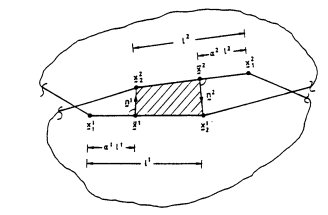
\includegraphics{Figure2/Chap4/fig7.png}
    \caption{Contact segment element}
   \label{fig4:7}
\end{figure}

Within this segment the displacement field and its variation is given as
\begin{equation}
\label{eqn:4.66}
\mathbf{u}^{\gamma}(\xi)=(1-\xi) \overline{\mathbf{u}}^{\gamma}+\xi \mathbf{u}_{2}^{\gamma} \quad \boldsymbol{\eta}^{\gamma}(\xi)=(1-\xi) \overline{\boldsymbol{\eta}}^{\gamma}+\xi \boldsymbol{\eta}_{2}^{\gamma}
\end{equation}
or the surface of the body $ \mathcal{B}^{\gamma}, \gamma=1,2 $. For the perturbed Lagrangian approach $ (38) $ the contact contributions take the form

\begin{equation}
\label{eqn:4.67}
\begin{aligned} \int_{\Gamma_{c}} \lambda_{N} \delta g_{N} d \Gamma &=\sum_{s=1}^{n_{s e g}} \int_{\Gamma_{s}} \lambda_{N} \delta g_{N} d \Gamma \\ \int_{\Gamma_{c}}\left(-\frac{\lambda_{N}}{\epsilon_{N}}+g_{N}\right) \delta \lambda_{N} d \Gamma &=\sum_{s=1}^{n_{s e g}} \int_{\Gamma_{s}}\left(-\frac{\lambda_{N}}{\epsilon_{N}}+g_{N}\right) \delta \lambda_{N} d \Gamma=0 \end{aligned} 
\end{equation}
where the latter equation can be solved for $ \lambda_{N} $ directly. With the interpolations $ (65) $ and assuming a constant contact pressure $ \lambda_{N} $ within the segment, $ \lambda_{N}=\bar{\lambda}_{N}=C O N S T . $, we obtain for the segment $ \Gamma_{s} $
\begin{equation}
\label{eqn:4.68}
\begin{aligned} \int_{\Gamma_{s}} \lambda_{N} \delta g_{N} d \Gamma &=\bar{\lambda}_{N} \int_{0}^{1}\left[\boldsymbol{\eta}^{1}(\xi)-\boldsymbol{\eta}^{2}(\xi)\right] \cdot \mathbf{n}(\xi)\left\|\frac{d \Gamma}{d \xi}\right\| d \xi \\ \int_{\Gamma_{s}}\left(-\frac{\lambda_{N}}{\epsilon_{N}}+g_{N}\right) \delta \lambda_{N} d \Gamma \Longrightarrow \bar{\lambda}_{N} &=\frac{\epsilon_{N}}{L_{s}} \int_{0}^{1}\left[\mathbf{u}^{1}(\xi)-\mathbf{u}^{2}(\xi)\right] \cdot \mathbf{n}(\xi)\left\|\frac{d \Gamma}{d \xi}\right\| d \xi \end{aligned}
\end{equation}
 The evaluation of these integrals by the trapezoidal rule yields the simple formulas
\begin{equation}
\begin{aligned}
\bar{\lambda}_{N} \int_{0}^{1}\left[\boldsymbol{\eta}^{1}(\xi)-\boldsymbol{\eta}^{2}(\xi)\right] \cdot \mathbf{n}(\xi)\left\|\frac{d \Gamma}{d \xi}\right\| d \xi & \approx \frac{1}{2} \bar{\lambda}_{N}\left(\left.\delta g_{N}\right|_{\xi=0}+\left.\delta g_{N}\right|_{\xi=1}\right) \\
\bar{\lambda}_{N} & \approx \frac{\epsilon_{N}}{2}\left(\left.g_{N}\right|_{\xi=0}+\left.g_{N}\right|_{\xi=1}\right)
\end{aligned}
\label{eqn:4.69}
\end{equation}
where $ g_{N} $ and $ \delta g_{N} $ can be expressed by the quantities in equations $ (\ref{eqn:4.65}) $ and $ (\ref{eqn:4.66}) $. This completes the discretization for contact segments. 


\subsection{ Global Set of Equations}
For a global algorithmic treatment we have to state the discrete set of equations. This leads for the penalty method to the general matrix formulation of the weak form
\begin{equation}
\mathbf{G}_{c}^{p}(\mathbf{v})=\mathbf{G}(\mathbf{v})+\cup_{s=1}^{n_{c}} \mathbf{G}_{s}^{c}(\mathbf{v})=\mathbf{0}
\label{eqn:4.70}
\end{equation}
where $ \mathbf{G}(\mathbf{v}) $ denotes the contributions of the bodies due to the weak form (43). In the second term $ s $ is associated with the active contact element, node or segment and $ \mathbf{G}_{s}^{c}(\varphi) $ has to be computed according to the chosen discretization, see previous sections. For the Lagrangian multiplier method the set of equations yields
\begin{equation}
\begin{array}{l}
\mathbf{G}_{c}^{1}(\mathbf{v}, \boldsymbol{\lambda})=\mathbf{G}(\mathbf{v})+\cup_{s=1}^{n_{c}} \mathbf{C}_{s}^{l}(\mathbf{v})^{T} \lambda_{s}=\mathbf{0} \\
\mathbf{G}_{c}^{2}(\mathbf{v}, \boldsymbol{\lambda})=\quad \cup_{s=1}^{n_{c}} \mathbf{C}_{s}^{g}(\mathbf{v}) \quad=\mathbf{0}
\end{array}
\label{eqn:4.71}
\end{equation}

Here the matrix $ C_{s}^{l}(\mathbf{v}) $ is related to the variation of $ \delta g_{s} $, see e.g. $ (\ref{eqn:4.68})_{1} $, and $ \mathbf{C}_{s}^{g}(\mathbf{v}) $ denotes the matrix formulation of the gap function $ g_{s} $ itself, see e.g. $ (\ref{eqn:4.68})_{2} $. These matrices also depend on the chosen discretization and are ment to contain not only the terms of the normal contact as indicated in (\ref{eqn:4.68}) but also the terms due to friction.

In case that Newton type methods are employed to solve $ (\ref{eqn:4.70}) $ or $ (\ref{eqn:4.71}) $ a linearization of the discrete set of equations has to be performed. Especially in the large deformation case the change in the normal has to be taken into account. 
\section{ ALGORITHMS FOR CONTACT PROBLEMS}

In this section we consider the algorithms which are essential for the treatment of contact problems. In general we have to distinguish between global algorithms which are necessary to find the correct number of active constraint equations and local algorithms which are needed to update contact stresses within the constitutive equations in the interface. Furthermore, also algorithms have to be deviced for coupled problems which may be necessary in case of thermomechanical coupling or for fluid-structure interaction problems.

The bandwidth of the global algorithms for constraint optimization is very broad. We like to mention, see also the introductory remarks, the simplex method, active set strategies, sequential quadratic programming, penalty and augmented Lagrangian techniques as well as barrier methods. All these techniques have advantages and disadvantages concerning efficiency, accuracy or robustness and thus have to be applied according to the problem
at hand. Algorithms for coupled problems, like staggered schemes, depend on the type of coupling and thus have to be designed with special care regarding robustness and efficiency. In the following we will sketch some of the global algorithms which are mainly applied to contact problems.

The update algorithms for the contact stresses, especially the tangential stresses due to friction, have been settled. In this case the so called projection methods or return mapping schemes yield the most efficient and robust treatment. Due to the fact that a algorithmic tangent operator can be constructed this technique can be incorporated in a Newton-Raphson scheme.

\subsection{ Global Algorithms}

The algorithm which is applied in many standard finite element programs is related to the penalty method. This is mainly due to its simplicity and furthermore it yields for many applications a robust algorithm. The penalty method is mostly combined with an active set strategy. The global set of equations is given in $ (\ref{eqn:4.70}) $. Now the algorithm for the penalty method can be summarized in here \\
\begin{framed}
Initialize algorithm \\
\ set: $ \mathbf{v}_{1}=\mathbf{0}, \quad \epsilon_{N}=\epsilon_{0} $\\
\hspace*{6mm} LOOP over iterations: $ i=1, \ldots $, convergence \\
\hspace*{10mm} Check for contact: $ g_{N s_{i}} \leq 0 \rightarrow $ active node, segment or element \\
 \hspace*{10mm} Solve: $ \mathbf{G}_{c}\left(\mathbf{v}_{i}\right)=\mathbf{G}\left(\mathbf{v}_{i}\right)+\cup_{s=1}^{n_{c}} \mathbf{G}_{s}^{c}\left(\mathbf{v}_{i}\right)=\mathbf{0} $ \\
 \hspace*{10mm} Check for convergence: $ \left\|\mathbf{G}_{c}\left(\mathbf{v}_{i}\right)\right\| \leq T O L \Rightarrow $ END LOOP \\
\hspace*{6mm}  END LOOP 
\\ update penalty parameter: $ \epsilon_{N} $
\end{framed}


Usually the solution of $ \mathbf{G}_{c}(\mathbf{v})=\mathbf{0} $ is performed by a Newton-Raphson iteration leading to
\begin{equation}
\label{eqn:4.72}
\begin{aligned}
D \mathbf{G}_{c}\left(\mathbf{v}_{i}^{n}\right) \Delta \mathbf{v}_{i}^{n+1} &=-\mathbf{G}_{c}\left(\mathbf{v}_{i}^{n}\right) \\
\mathbf{v}_{i}^{n+1} &=\mathbf{v}_{i}^{n}+\Delta \mathbf{v}_{i}^{n+1}
\end{aligned}
\end{equation}

where the operator $ D $ denotes the directional derivative of the vector $ \mathbf{G}_{c}\left(\mathbf{v}_{i}^{n}\right) $ which results in the tangent matrix $ \mathbf{K}_{T}\left(\mathbf{v}_{i}^{n}\right)=D \mathbf{G}_{c}\left(\mathbf{v}_{i}^{n}\right) $. The iteration index $ n $ is related to the Newton loop to solve $ \mathbf{G}_{c}\left(\mathbf{v}_{i}\right)=\mathbf{0} $ in Box 1 . Often the active set strategy, stated in Box 1, is accelerated in such a way that the update of the active set of contact constraints is performed within each step in the Newton iteration. Then the iteration $ (72) $ yields
\begin{equation}
\label{eqn:4.73}
 \begin{aligned} D \mathbf{G}_{c}\left(\mathbf{v}_{i}\right) \Delta \mathbf{v}_{i+1} &=-\mathbf{G}_{c}\left(\mathbf{v}_{i}\right) \\ \mathbf{v}_{i+1} &=\mathbf{v}_{i}+\Delta \mathbf{v}_{i+1} \end{aligned} 
\end{equation}
which is considerably faster. However this procedure might not converge for all cases and thus has to be applied with care.

Within this algorithm, an increase of the penalty parameter is necessary when the final result shows visible penetrations and thus does not fulfill the constraint equation $ g_{n+}=0 $ in a correct way. On the other hand a penalty parameter which has been chosen
too large can lead to ill-conditioning of the equation system and thus has to be reduced to avoid this. On possibility for the choice of $ \epsilon_{N} $ is to relate the penalty parameter to the bulk modulus of the contacting bodies. However, since it is quite hard to estimate the penalty parameter for all cases it makes sense to apply the augmented Lagrangian technique.

Augmented Lagrangian technique are usually applied together with Uzawa type algorithms, see Bertsekas (1984), Glowinski, Le Tallec (1984) or Laursen, Simo (1991), which lead to an inner loop for the contact and an outer loop for the update of the Lagrangian parameters.



Let us remark that it is standard practice in augmented Lagrangian iterations also to update the penalty number $ \epsilon_{N} $ in order to obtain good convergence, see Bertsekas (1984). This is due to the fact that a small penalty parameter leads to very slow convergence since the update formula (42) is of first order and the contact forces due to the penalty are small. Thus it makes sense to increase the penalty parameter within a contact element $ s $ according to an update scheme, see Bertsekas (1984). Here we like to show this approach for the augmented Lagrangian scheme in combination with constitutive interface laws like (13). The update scheme yields
\begin{equation}
\label{eqn:4.74}
 \epsilon_{N s n+1}=\left\{\begin{array}{ll}10 \cdot \epsilon_{N s n} & \text { for }\left[c_{+}\left(\mathbf{V}_{s}, \bar{P}_{N s}\right)\right]_{n+1}>\frac{1}{4} \cdot\left[c_{+}\left(\mathbf{V}_{s}, \bar{P}_{N s}\right)\right]_{n} \text { and } \epsilon_{N s n} \leq \frac{k}{\sqrt{N t}} \\ \epsilon_{N s n} & \text { for }\left[c_{+}\left(\mathbf{V}_{s}, \bar{P}_{N s}\right)\right]_{n+1} \leq \frac{1}{4} \cdot\left[c_{+}\left(\mathbf{V}_{s}, \bar{P}_{N s}\right)\right]_{n}\end{array}\right. 
\end{equation}

In relation (\ref{eqn:4.74}) also a stopping criterion for the update of the penalty parameter has been introduced to avoid ill-conditioning. This is given by the estimate (39). The global augmented Lagrangian algorithm is shown in box bellow. Here we use again the discrete formulation (70) which has to be adjusted to incorporate the fixed Lagrangian parameters $ \bar{P}_{N s} $, see $ (62) $ for the node-to-segment discretization. By $ \cup_{s=1}^{n_{c}} \mathbf{G}_{s n+1}^{a}\left(\mathbf{v}, \bar{P}_{N s}\right) $ we denote the contribution of the fourth term in (41) for an active contact element $ s $.
\begin{framed}
    Initialize algorithm\\
    set: $ d_{0}=\xi, \quad \mathbf{v}=\mathbf{0}, \quad \bar{P}_{0}=0, \quad \epsilon_{N}=\epsilon_{N 0} $\\
LOOP over augmentations: $ n=1, . . $, convergence \\
\hspace*{6mm} LOOP over iterations : $ i=1, . . $  convergence\\
\hspace*{10mm} Solve: $ \mathbf{G}_{c}\left(\mathbf{v}_{i},\\ \bar{P}_{N_{n}}\right)=\mathbf{G}\left(\mathbf{v}_{i}\right)+\cup_{s=1}^{n_{c}} \mathbf{G}_{s n+1}^{a}=\mathbf{0} $\\
\hspace*{10mm} Check for convergence: $ \left\|\mathbf{G}_{c}\left(\mathbf{v}_{i}, \bar{P}_{N_{n}}\right)\right\| \leq T O L \Rightarrow $  END LOOP\\
\hspace*{6mm} END LOOP\\
\hspace*{6mm} LOOP over contact nodes : $s = 1,\dots, n_c$\\
\hspace*{10mm} Update: $\bar{P}_{N_{s} n+1}$ according to $(62)$ \\
\hspace*{10mm} Update: $d_{s n+1}=h\left(\bar{P}_{N_{s n+1}}\right)$ according to (12) \\
\hspace*{10mm} Update: $\epsilon_{N s n+1}$ according to $(74)$\\
\hspace*{10mm} Check for convergence: $ \frac{1}{\zeta}\left\|g_{N_{+}}\left(\mathbf{V}_{s i}\right)-\left(\zeta-d_{n+1}\right)\right\| \leq T O L \Rightarrow S T O P $\\
\hspace*{6mm} END LOOP\\
END LOOP \\ 
\end{framed}

% \input{Page/Chap4/29}
% \input{Page/Chap4/30}